
\hypertarget{working_searchinfiles}{}
\section{Search in files}
\index{search!in files}

\begin{figure}[h!]
  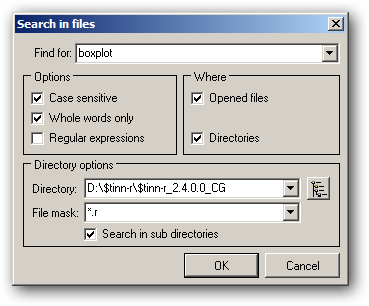
\includegraphics[scale=0.35]{./res/searchinfiles.png}~~
  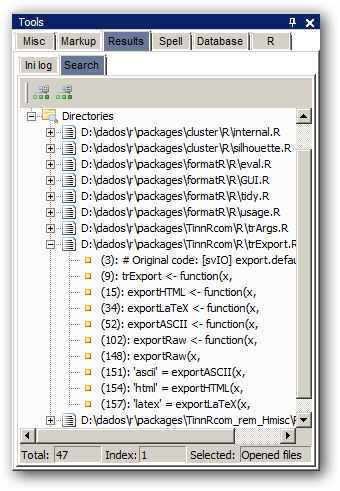
\includegraphics[scale=0.35]{./res/tools_results_search.png}\\
  \caption{Search in files.}
  \label{fig:searchinfiles}
\end{figure}


The \textit{Search in files} dialog
(Figure \ref{fig:searchinfiles})
allows you to match a criteria in all opened files and/or in files on disk.


\subsection{Options}
\index{search!case sensitivity}
\index{search!regular expressions}

\begin{quote}
  \begin{footnotesize}
    \begin{description}
      \item[Case sensitive:]
        When this option is set the search is case sensitive.
        For example, \texttt{Ab}, \texttt{AB} and \texttt{ab}
        are all treated as different words.
      \item[Whole words only:]
        When this option is set the system will only find complete
        words matching the search criteria. For example, if
        \texttt{ab} is the search string the system will not match
        occurrences of words such as \texttt{abc} or \texttt{cab}.
      \item[Regular expressions:]
        \htmladdnormallink{See regular expressions ...}{\#working\_regularexpressions}
    \end{description}
  \end{footnotesize}
\end{quote}


\subsection{Where}
\begin{quote}
  \begin{footnotesize}
    \begin{description}
      \item[Opened files:]
        When this option is set the search is performed on all opened files.
      \item[Directories:]
        When this option is set the search is performed in disk files.
    \end{description}
  \end{footnotesize}
\end{quote}


\subsection{Directory options}
\begin{quote}
  \begin{footnotesize}
    \begin{description}
      \item[Directory:]
        A dropdown list of previously searched directories.
      \item[File mask:]
        A dropdown list of the previously searched file mask.
      \item[Search in sub directories:]
        When this option is set the search is performed on all sub
        directories of the main directory.
    \end{description}
  \end{footnotesize}
\end{quote}


\subsection{Results interface}
The associated results interface
(Figure \ref{fig:searchinfiles})
shows the results.

A double click in a single occurrence (or dragging and dropping it into the
editor interface) will open the file and results will be placed in the first
line of the editor window.
